\documentclass[a4paper,10pt]{jsarticle}
\usepackage{color}
\usepackage[dvipdfmx]{graphicx}
\usepackage{amsmath}

\author{sankaku}
\date{\today}
\title{otofu sample}

\begin{document}
\maketitle

\section{通常は表示できない文字}
\label{通常は変換できない文字のセクション}

髙

﨑

閒

礴

搢

婭

鷗

①②③④⑤⑥⑦⑧⑨⑩

ⅠⅡⅢⅣⅤⅥⅦⅧⅨⅩ

\section{コメントのセクション}
\label{コメントのセクション}

% ここはコメントです。

%ここもコメントです。

\% ここはコメントではありません。% ここはコメントです。

% 次のファイルにはアクセスしません。\input{foo/bar/baz.tex}

\section{includeなど}
\label{includeなどのセクション}

main.texからsub1.texをincludeします。

これはmain.texで参照されているファイルsub1.texです。

髙

﨑

閒

礴

搢

婭

鷗

①②③④⑤⑥⑦⑧⑨⑩

ⅠⅡⅢⅣⅤⅥⅦⅧⅨⅩ

sub1.texここまで。


main.texからsub2.texをinputします。

これはmain.texで参照されているファイルsub2.texです。

\subsection{通常は表示できない文字 subsub1}
\label{通常は変換できない文字のセクション subsub1}
dir/subsub1.texをinputします。

これはsub2.texで参照されているファイルdir/subsub1.texです。

髙

﨑

閒

礴

搢

婭

鷗

①②③④⑤⑥⑦⑧⑨⑩

ⅠⅡⅢⅣⅤⅥⅦⅧⅨⅩ

dir/subsub1.texここまで。


sub2.texここまで。


\section{includegraphicsなど}
\label{includegraphicsなどのセクション}


main.texからdir/graph.texをinputします。

これはmain.texで参照されているファイルdir/graph.texです。


画像サンプル: \includegraphics[width=1cm]{img/not/converted.eps}

これはコマンドではない: \\includegraphics[width=1cm]{img/not/converted.eps}

コマンド部だけ変換される \\includegraphics[width=1cm]{\includegraphics[width=1cm]{img/not/converted.eps}}


%画像サンプル: \includegraphics[width=1cm]{img/ここは/変換/されない.eps}

これはコマンドではない: \\includegraphics[width=1cm]{img/ここは/変換/される.eps}

%コマンド部だけ変換される \\includegraphics[width=1cm]{\includegraphics[width=1cm]{img/ここは/変換/されない.eps}}

dir/graph.texここまで。



\section{refのセクション}
\label{refのセクション}

\ref{通常は変換できない文字のセクション}、\ref{includeなどのセクション}、\ref{includegraphicsなどのセクション}、\ref{refのセクション}を参照のこと。

\end{document}

